%  article.tex (Version 3.3, released 19 January 2008)
%  Article to demonstrate format for SPIE Proceedings
%  Special instructions are included in this file after the
%  symbol %>>>>
%  Numerous commands are commented out, but included to show how
%  to effect various options, e.g., to print page numbers, etc.
%  This LaTeX source file is composed for LaTeX2e.

%  The following commands have been added in the SPIE class 
%  file (spie.cls) and will not be understood in other classes:
%  \supit{}, \authorinfo{}, \skiplinehalf, \keywords{}
%  The bibliography style file is called spiebib.bst, 
%  which replaces the standard style unstr.bst.  

\documentclass[]{spie}  %>>> use for US letter paper
%%\documentclass[a4paper]{spie}  %>>> use this instead for A4 paper
%%\documentclass[nocompress]{spie}  %>>> to avoid compression of citations
%% \addtolength{\voffset}{9mm}   %>>> moves text field down
%% \renewcommand{\baselinestretch}{1.65}   %>>> 1.65 for double spacing, 1.25 for 1.5 spacing 
%  The following command loads a graphics package to include images 
%  in the document. It may be necessary to specify a DVI driver option,
%  e.g., [dvips], but that may be inappropriate for some LaTeX 
%  installations. 
\usepackage[]{graphicx}

\usepackage[utf8x]{inputenc}	% polish letters (for names)
\usepackage{mathtools}			% matrix*
\usepackage{booktabs}			% professional tables
\usepackage[]{amsmath}
\usepackage{listings}
\usepackage[usenames,dvipsnames]{xcolor} % listing colors

\lstdefinestyle{outcode}
{
basicstyle={\footnotesize},
keywordstyle={\bf\footnotesize\color{black}},
commentstyle={\em\footnotesize\color{gray}},
numbers=left,
stepnumber=5,
firstnumber=1,
numberfirstline=true,
numberblanklines=true,
numberstyle={\sf\tiny},
numbersep=10pt,
tabsize=2,
xleftmargin=17pt,
framexleftmargin=3pt,
framexbottommargin=2pt,
framextopmargin=2pt,
framexrightmargin=0pt,
showstringspaces=true,
extendedchars=true,
% title=\lstname,
captionpos=b,
% abovecaptionskip=1pt,
% belowcaptionskip=1pt,
frame=tb,
framerule=0.1pt,
breaklines=true,
}

\newcommand{\bm}[1]{\boldsymbol{#1}}

\title{Implementation aspects of Graph Neural Networks}

%>>>> The author is responsible for formatting the 
%  author list and their institutions.  Use  \skiplinehalf 
%  to separate author list from addresses and between each address.
%  The correspondence between each author and his/her address
%  can be indicated with a superscript in italics, 
%  which is easily obtained with \supit{}.


\author{
Barcz A.\supit{a}, Szymański Z.\supit{a}, Jankowski S.\supit{b}
\skiplinehalf
\supit{a}Warsaw University of Technology, Institute of Computer Science;\\
\supit{b}Warsaw University of Technology, Institute of Electronic Systems
}

%>>>> Further information about the authors, other than their 
%  institution and addresses, should be included as a footnote, 
%  which is facilitated by the \authorinfo{} command.

\authorinfo{(abarcz@gmail.com, z.szymanski@ii.pw.edu.pl, s.jankowski@ise.pw.edu.pl)}
%%>>>> when using amstex, you need to use @@ instead of @
 

%%%%%%%%%%%%%%%%%%%%%%%%%%%%%%%%%%%%%%%%%%%%%%%%%%%%%%%%%%%%% 
%>>>> uncomment following for page numbers
% \pagestyle{plain}    
%>>>> uncomment following to start page numbering at 301 
%\setcounter{page}{301} 
 
\begin{document} 
\maketitle 

%%%%%%%%%%%%%%%%%%%%%%%%%%%%%%%%%%%%%%%%%%%%%%%%%%%%%%%%%%%%% 
\begin{abstract}
This article summarises the results of implementation of a Graph Neural Network~\cite{scarselli2009graph} classifier. The Graph Neural Network model is a quite recent connectionist model, capable of processing various types of structured data, including nonpositional and cyclic graphs. To operate correctly, the GNN model must implement a transition function being a contraction map, which is assured by imposing a penalty on model weights. This article presents some preliminary results concerning the impact of the penalty parameter on the model training process and the practical decisions that were made during the GNN implementation process.
\end{abstract}

%>>>> Include a list of keywords after the abstract 

\keywords{Graph Neural Network, GNN, graph, classification, contraction map}

%%%%%%%%%%%%%%%%%%%%%%%%%%%%%%%%%%%%%%%%%%%%%%%%%%%%%%%%%%%%%
\section{Introduction}
A Graph Neural Network model~\cite{scarselli2009graph} is a connectionist model capable of performing classification and regression on structured data. The structure of such data usually contains important information, which would be lost after converting the data to plain vector representation. Several methods were devised to process structured data, including graph kernels, inductive logic programming, probabilistic models, evolutionary algorithms and connectionist models. The area of interest of this article are the connectionist models, which are based on neural networks. Since the first connectionist models were created (the RAAM~\cite{pollack1990recursive} and LRAAM~\cite{sperduti1994labelling} models), it was shown that providing a classifier with explicit information about data structure yields better results that ignoring that information or encoding it in a predefined way. Later on, two important rules were devised. Firstly for a given structured dataset its \emph{representation should be learned, instead of being handcrafted}~\cite{goulon2005hopfield}. That is, machine learning should be used to transform structured data into a meaningful representation, which should either encode all the information present in the data, or only the part that is important for a classification/regression task. Secondly, \emph{the structure of a classifier should reflect the structure of data being processed}~\cite{goulon2005hopfield}. That is, classifiers that are built of units connected according to the processed graph topology perform better than the non-structured ones. The main limitation of most connectionist models was that they were able to process only a certain class of graphs, namely directed positional acyclic graphs (DPAGs). Cyclic graphs could be processed only after a preprocessing phase. That phase could consist of e.g. deleting cycles and storing information about them in labels~\cite{goulon2005learning},  introducing a delay in the case of LRAAM~\cite{goulon2005hopfield} or converting the graphs to \emph{recursive equivalent} trees~\cite{bianchini2003backpropagation}. Nonpositional graphs were processed by introducing a predefined order of the children of a node, like in the case of chemical compounds~\cite{ivanciuc2003canonical}. A distinct feature of the GNN model is that it is capable of directly processing almost all types of graphs, including nonpositional and cyclic ones. No preprocessing, which could possibly lead to some data loss, is necessary. The GNN model is similar to the recursive neural networks model~\cite{frasconi1998general}, which could be applied to both positional and nonpositional graphs~\cite{bianchini2005recursive}. The GNN model, however, introduced a novel backpropagation scheme, which allows processing cyclic graphs in a straightforward manner. The GNN model was successfully applied in the field of XML document processing~\cite{yong2006xml}, image classification~\cite{quek2011structural}, object localisation~\cite{monfardini2006graph} and web page ranking~\cite{scarselli2005graph}. This article describes an implementation of a Graph Neural Network classifier, highlighting the decisions that were made to produce an efficient and reliable classifier. The classifier was implemented using GNU Octave. The classifier was implemented to be as general as possible, capable of processing all the graph types mentioned in the original article~\cite{scarselli2009graph}. An important parameter of the model, the \emph{contraction constant} parameter $\mu$ and its impact on the process of learning was described. Some preliminary results were presented, suggesting that for a given dataset there exists a minimal value of $\mu$ and that value determines if any learning will occur.

\section{Input data}
The input data for the classifier consisted of a set of graphs or a single graph. As disconnected graphs were allowed, a set of graphs could easily be converted to a single large disconnected graph, which was then fed to the classifier. Each input graph consisted of: node labels (for a single node $n$ its label was $\bm{l}_n, |\bm{l}_n| \geq 1$), edge labels (for a directed edge from node $u$ to node $n$ its label was $\bm{l}_{(n,u)}, |\bm{l}_{(n,u)}| \geq 0$) and node outputs (for a single node $n$ its output was $\bm{o}_n, |\bm{o}_n| \geq 1$). To distinguish between directed and undirected edges a method different from the original one was implemented. A directed edge usually means that each of its nodes influence the other one equally. An undirected edge suggests that the influence is unidirectional. Therefore directed edges were represented as pairs of undirected edges, so the bidirectional relation could be represented explicitly.

\section{Computation units}
A GNN classifier consists of two separate computation units: $f_{\bm{w}}$ and $g_{\bm{w}}$. The $f_{\bm{w}}$ unit (the local \emph{transition function}) builds for each node $n$ its representation $\bm{x}_n$ (the \emph{state}). The $g_{\bm{w}}$ unit (the local \emph{output function}) takes as input the obtained node representation, producing result that should match the expected output $\bm{o}_n$ for the $n$th node. For this implementation the nonpositional form of $f_{\bm{w}}$ was chosen as the more general one and the one performing better at various tasks~\cite{scarselli2009graph}. To assure that the classifier implemented was capable of building a sufficient representation, a minimal form of $f_{\bm{w}}$ and $g_{\bm{w}}$ was chosen as shown in Eq.~\ref{eq:hw} and Eq.~\ref{eq:gw}. The $f_{\bm{w}}$ unit was implemented as a simple sum of the $h_{\bm{w}}$ unit outputs evaluated at each directed edge $(n, u)$, connecting node $u$ to the node $n$. All instances of the $h_{\bm{w}}$ unit shared their weights and all instances of the $g_{\bm{w}}$ unit shared their weights. 

\begin{equation}
\bm{x}_n = \sum_{u \in ne[n]} h_{\bm{w}}(\bm{l}_n, \bm{l}_{(n, u)}, \bm{x}_u)
\label{eq:hw}
\end{equation}

\begin{equation}
\bm{o}_n = g_{\bm{w}}(\bm{x}_n)
\label{eq:gw}
\end{equation}

\begin{figure}[h!]
\begin{center}
	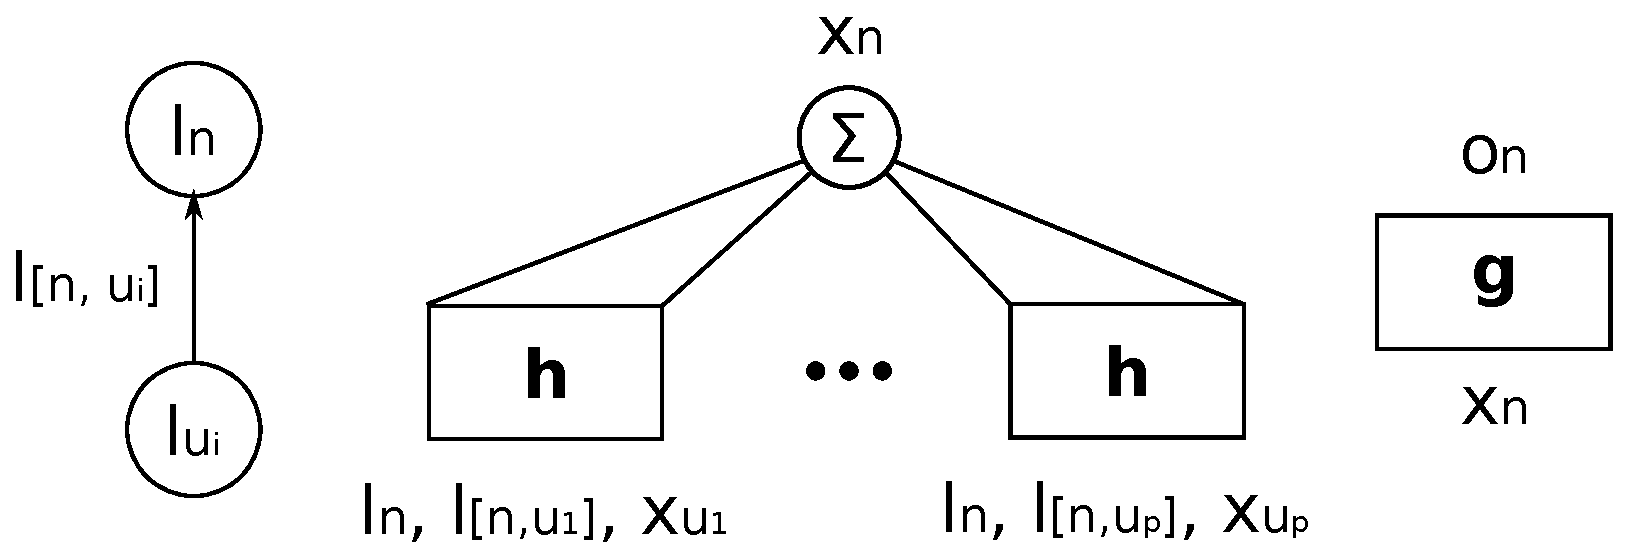
\includegraphics[scale=0.4]{img/f_ext2}
	\caption{The $f_{\bm{w}}$ unit for a single node, one of the corresponding edges and the $g_{\bm{w}}$ unit}
	\label{fig:gnn_f}
\end{center}
\end{figure}

Both $h_{\bm{w}}$ and $g_{\bm{w}}$ units were implemented as three layer feed-forward neural networks (inputs, hidden layer, output layer). In both units the hidden layers were composed of $tanh$ neurons. In the $h_{\bm{w}}$ unit the output layer was composed of $tanh$ neurons to assure that the state $\bm{x}_n$, which was later passed to the $g_{\bm{w}}$ network, consisted of bounded values only. The output layer of the $g_{\bm{w}}$ unit could be configured either as a layer with $tanh$ activation function or a layer of linear neurons. The weights of both the $h_{\bm{w}}$ and $g_{\bm{w}}$ units were initialised according to standard neural network practice, to avoid saturation of any $tanh$ activation function: $net_j = \sum_i w_{ji} y_i \in (-1, 1)$, where $net_j$ is the input to $j$th neuron activation function, $y_i$ is the $i$th input and $w_{ji}$ is the weight on the corresponding connection. The initial input weights of the $g_{\bm{w}}$ unit were divided by an additional factor, i.e. the maximum node indegree of the processed graphs, to reflect the fact, that the input of $g_{\bm{w}}$ unit consists of a sum of $h_{\bm{w}}$ outputs. All input data (node and edge labels) was normalised appropriately.

\section{Encoding network and the training algorithm}
A network of identical $f_{\bm{w}}$ units, connected according to the processed graph topology forms an \emph{encoding network}. The encoding network is used to build the graph nodes representation $\bm{x}$ (set of all single node representations $\bm{x}_n$) which is later used to calculate the nodes output $\bm{o}$ (set of all single node outputs $\bm{o}_n$). A sample graph with its encoding network was presented in Fig.~\ref{fig:graphenc}. Let's denote by $F_{\bm{w}}$ the \emph{global transition function}, implemented by the encoding network and by $G_{\bm{w}}$ the \emph{global output function}, which produces the output. Let's denote by $l$ the set of all node and edge labels from a graph. The GNN training algorithm was implemented as follows:
\begin{enumerate}
	\item initialize $h_{\bm{w}}$ and $g_{\bm{w}}$ weights
	\item until stop criterion is satisfied:
	\begin{enumerate}
		\item initialize $\bm{x}$ randomly
		\item FORWARD: calculate $\bm{x} = F_{\bm{w}}(\bm{l}, \; \bm{x})$ until convergence
		\item BACKWARD: calculate $\bm{o} = G_{\bm{w}}(\bm{x})$ and backpropagate the error
		\item update $h_{\bm{w}}$ and $g_{\bm{w}}$ weights
	\end{enumerate}
\end{enumerate}
\noindent The stop criterion implemented was a maximum number of iterations.

\begin{figure}[h!]
\begin{center}
	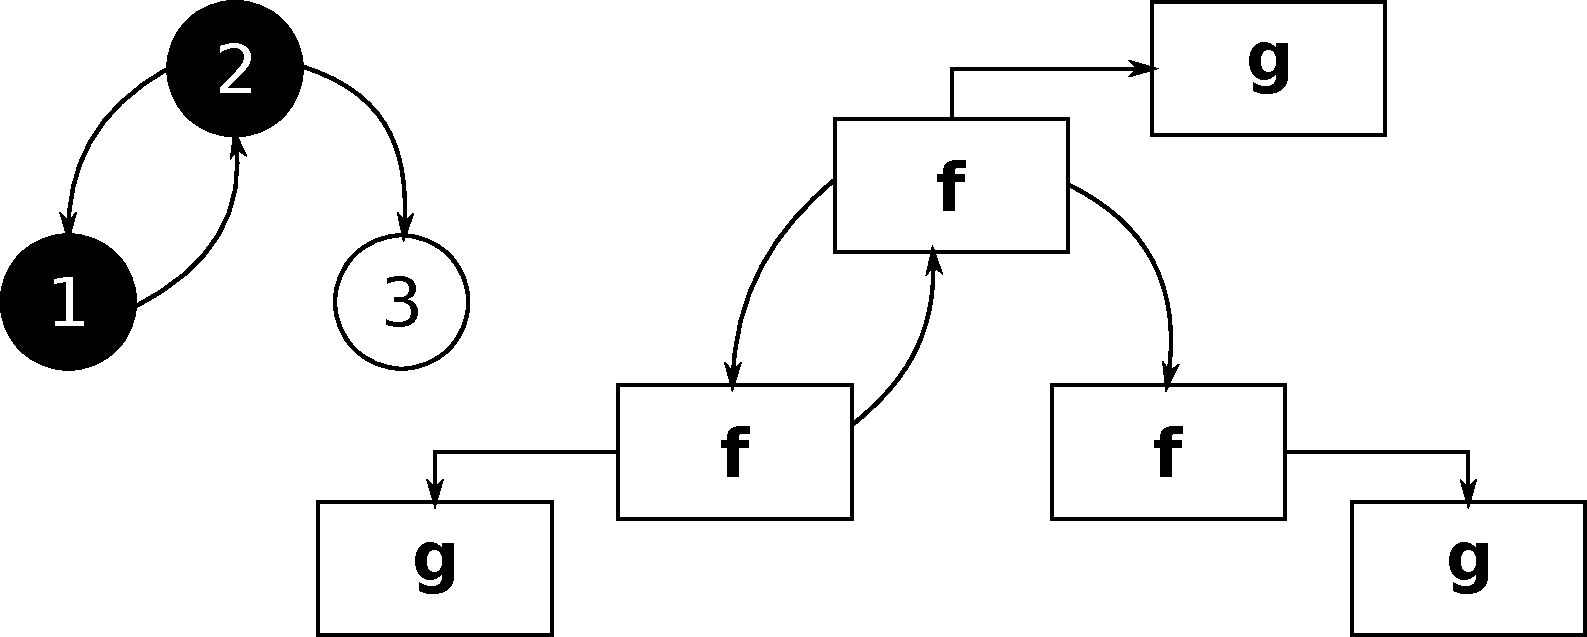
\includegraphics[scale=0.4]{img/graphenc}
	\caption{Sample graph with nodes belonging to two classes and the corresponding encoding network}
	\label{fig:graphenc}
\end{center}
\end{figure}

\subsection{Forward}
The computation of fixed point $\bm{x}$ was implemented according to the original source. The encoding network was unfolded in time up to a point, where the state reached fixed point. The process of reaching convergence in computation of the state can be viewed as performing time steps, where at each time step $f_{\bm{w}}$ is evaluated at each node of the graph and the graph edges are taken into consideration only between time steps~(Fig.~\ref{fig:forward}). Random initialisation of the state $\bm{x}$ at the beginning of each FORWARD call proved to work well. However, number of steps necessary to reach fixed point could vary a lot - from about 5 to 40 steps when $F_{\bm{w}}$ was indeed a contraction map to several thousands and probably more (computation was interrupted due to excessive time) when $F_{\bm{w}}$ was losing its contraction features. Therefore, for the sake of conducting experiments in predictable time, a maximum number of steps for the unfolding phase was introduced (\emph{maxForwardSteps}) and set to 200 for all the subsequent experiments. This value was chosen to be significantly larger than the usual number of steps made by the FORWARD procedure during the experiments, to allow reaching the fixed point if possible. It was observed that even when the algorithm reached the maximum number of steps and the calculation of $\bm{x}$ was interrupted (and therefore not exact), the learning algorithm was still able to perform quite well. In most cases, the RMSE error didn't increase significantly or even continued to drop.


\subsection{Backward}
The error backpropagation algorithm was implemented according to the original source, in a way similar to the Almeida-Pineda algorithm~\cite{williams1995gradient} designed for BPTT. The error of the $g_{\bm{w}}$ units was calculated, backpropagated through the unfolded network and also injected at each time step (Fig.~\ref{fig:backward}). In such way every "layer" of $f_{\bm{w}}$ units at a given time step $t_i$ was provided with two kinds of error - an error backpropagated through the subsequent time steps of the unfolded network and also an error coming directly from the $g_{\bm{w}}$ units, as if the unfolding had been stopped after the time step $t_i$. By using the Almeida-Pineda algorithm, the error was actually calculated recurrently up to a point, when the error accumulator value reached fixed point. The initial value of the error accumulator $z_0$ was set to the error backpropagated through the $g_{\bm{w}}$ layer. To assure a predictable computation time, a maximum number of steps for error accumulation was introduced (\emph{maxBackwardSteps}) and set to 200, just like in the case of the maximum number of forward steps. However, the actual number of backward steps proved to be much smaller than the number of forward steps and rarely reached the maximum value.

\begin{figure}[h!]
\begin{center}
	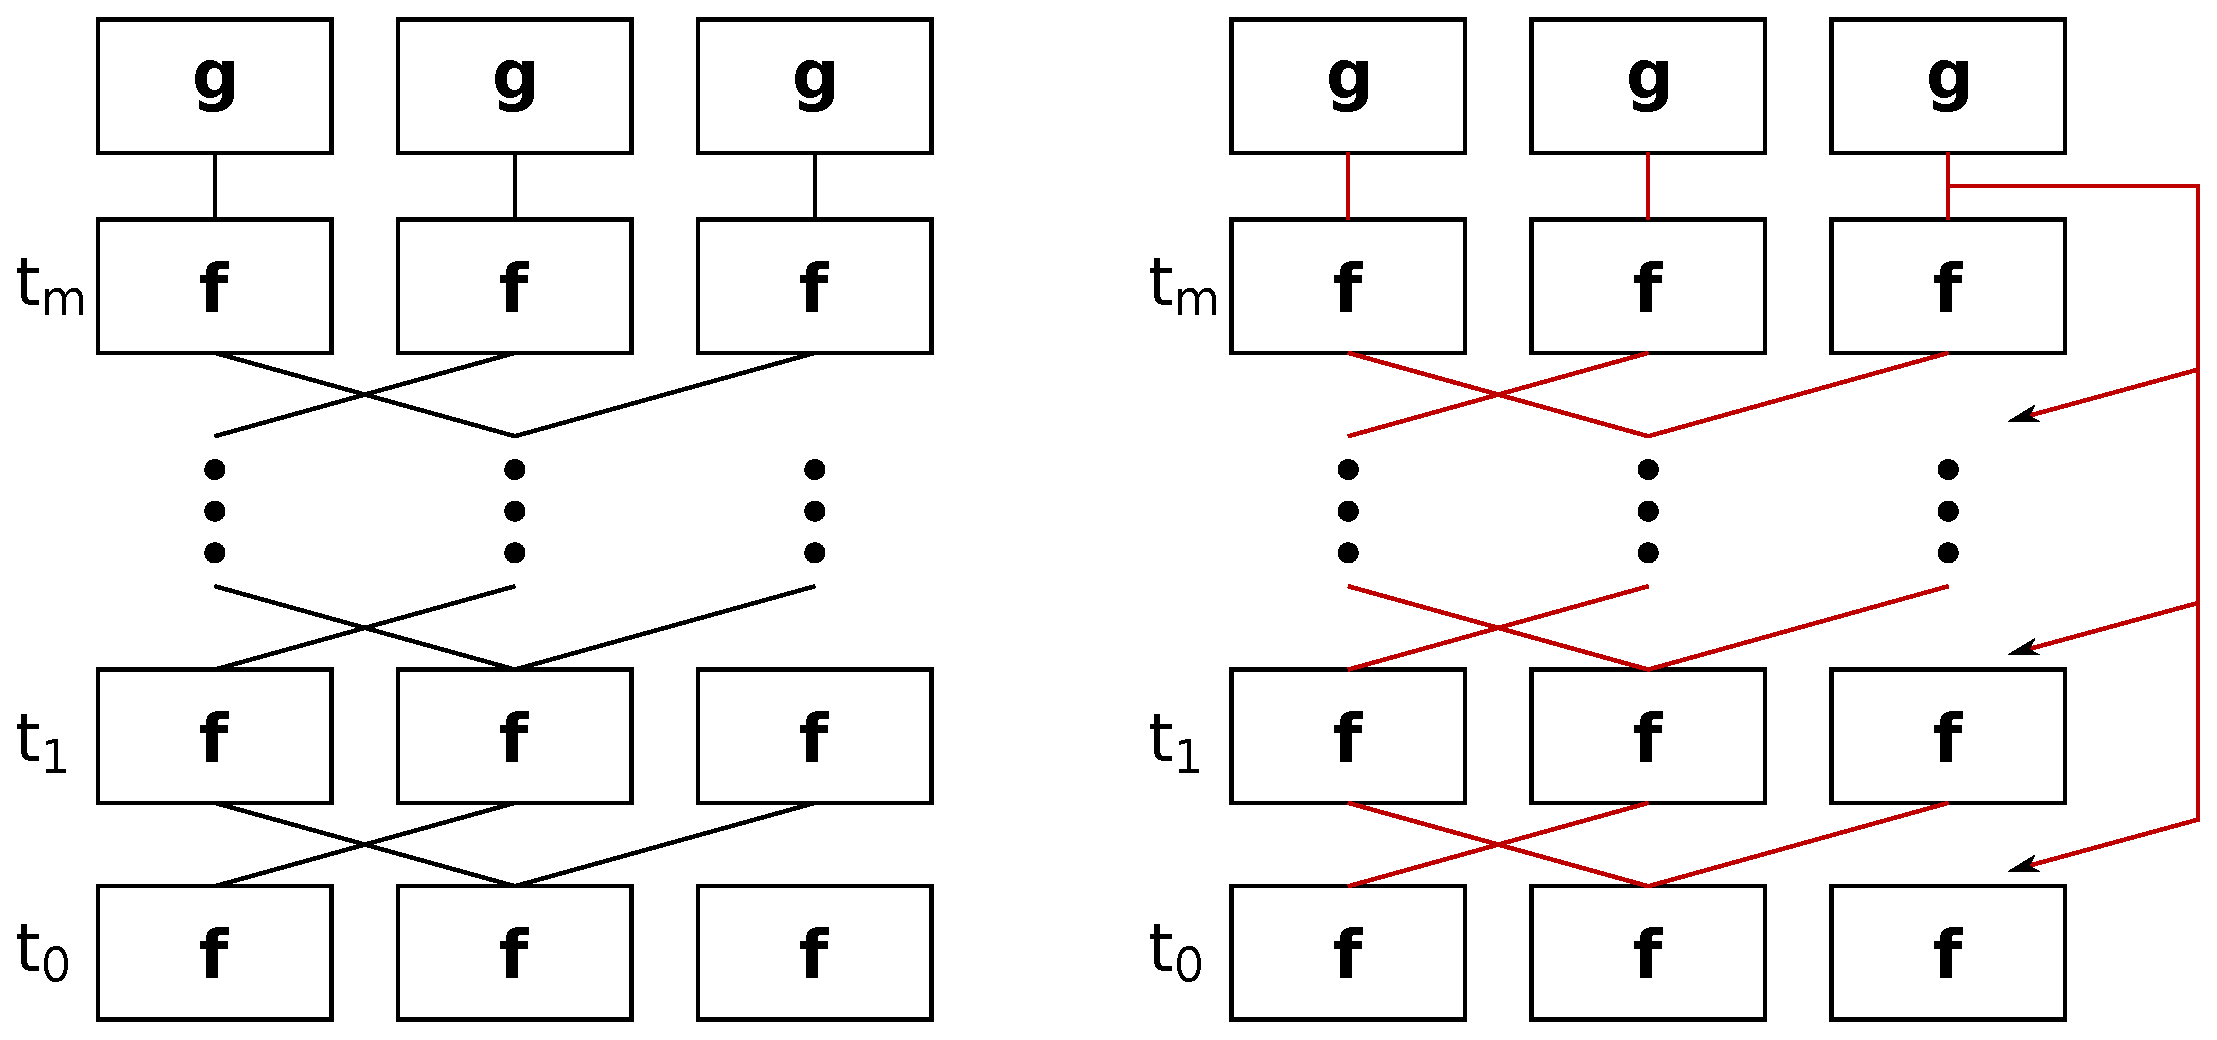
\includegraphics[scale=0.4]{img/forback}
	\caption{Encoding network unfolded and error backpropagation}
	\label{fig:forward}
	\label{fig:backward}
\end{center}
\end{figure}

\subsection{RPROP algorithm}
The BACKWARD procedure produces two kinds of weight updates: $\frac{\partial e_{\bm{w}}}{\partial \bm{w}}$ and $\frac{\partial p_{\bm{w}}}{\partial \bm{w}}$. The first is the error calculated by Almeida-Pineda algorithm for $h_{\bm{w}}$ and $g_{\bm{w}}$. The second is the derivative of penalty imposed on $h_{\bm{w}}$~weights to make $F_{\bm{w}}$ a contraction map, when $F_{\bm{w}}$ ceases to be one. The corresponding $\frac{\partial e_{\bm{w}}}{\partial \bm{w}}$ and $\frac{\partial p_{\bm{w}}}{\partial \bm{w}}$ errors are summed up to form the final weight update which would normally be used to update the weights in a standard neural network learning algorithm. However, it occurred that the term $\frac{\partial p_{\bm{w}}}{\partial \bm{w}}$ was sometimes several orders of magnitude larger than the $\frac{\partial e_{\bm{w}}}{\partial \bm{w}}$ term, a disproportion that could render the traditional gradient descent algorithm useless. Therefore the RPROP algorithm had to be used, not only to make the gradient descent fast~\cite{scarselli2009graph}, but also to make it robust against the potentially unforeseeable behaviour of the  $\frac{\partial e_{\bm{w}}}{\partial \bm{w}}$ term. Some experiments with the standard gradient descent algorithm confirmed that when $\frac{\partial p_{\bm{w}}}{\partial \bm{w}}$ was applied directly to weights, the learning algorithm couldn't reach its target. Introducing the RPROP algorithm fixed that issue, as the algorithm uses only the sign of the original weight updates and discards their values. Based on that sign, the algorithm calculates its own weight updates, which are adjusted to assure fast descent on steep gradient slopes and small modifications in the proximity of a function minimum. The RPROP algorithm was configured using standard recommended values~\cite{riedmiller1993direct}, with the exception of $\Delta_{max}$ which was set to $1$ to avoid large weight changes. 

\newpage
\subsection{Detailed training algorithm}
\begin{lstlisting}[mathescape, style=outcode, language=pascal, caption=The learning algorithm]
MAIN:
	$\bm{w} = \text{initialize}$
	$\bm{x} = FORWARD(\bm{w})$
	for $numberOfIterations$:
		$[\frac{\partial eh_{\bm{w}}}{\partial \bm{w}}; \; \frac{\partial eg_{\bm{w}}}{\partial \bm{w}}] = BACKWARD(\bm{x}, \; \bm{w})$
		$\bm{w} = \text{rprop-update}(\bm{w}, \; \frac{\partial eh_{\bm{w}}}{\partial \bm{w}}, \; \frac{\partial eg_{\bm{w}}}{\partial \bm{w}})$
		$\bm{x} = FORWARD(\bm{w})$
	end
	return $\bm{w}$
end

FORWARD($\bm{w}$):
	$\bm{x}(0) = \text{random}$
	$t = 0$
	repeat:
		$\bm{x}(t+1) = F_{\bm{w}}(\bm{x}(t), \; \bm{l})$
		$t = t + 1$
	until $(max_i(|x_i(t + 1) - x_i(t)|) \leq minStateDiff)$ or $(t > maxForwardSteps)$
	return $\bm{x}(t)$
end

BACKWARD($\bm{x}$, $\bm{w}$):
	$\bm{o} = G_{\bm{w}}(\bm{x})$
	$\bm{A} = \frac{\partial F_{\bm{w}}}{\partial \bm{x}}(\bm{x}, \; \bm{l})$
	$\bm{b} = \frac{\partial e_{\bm{w}}}{\partial \bm{o}}\cdot \frac{\partial G_{\bm{w}}}{\partial x}(\bm{x})$
	$\bm{z}(0) = \bm{b}$
	$t = 0$
	repeat:
		$\bm{z}(t - 1) = \bm{z}(t) \cdot \bm{A} + \bm{b}$
		$t = t - 1$
	until $(max_i(|z_i(t - 1) - z_i(t)|) \leq minErrorAccDiff)$ or $(|t| > maxBackwardSteps)$
	$\frac{\partial eg_{\bm{w}}}{\partial \bm{w}} = b$
	$\frac{\partial eh_{\bm{w}}}{\partial \bm{w}} = \bm{z}(t) \cdot \frac{\partial F_{\bm{w}}}{\partial \bm{w}}(\bm{x}, \bm{l}) + \frac{\partial p_{\bm{w}}}{\partial \bm{w}}$
	return $[\frac{\partial eh_{\bm{w}}}{\partial \bm{w}}; \; \frac{\partial eg_{\bm{w}}}{\partial \bm{w}}]$
end
\end{lstlisting}

\section{Influence of the contraction constant}
Weights of the $h_{\bm{w}}$ unit were penalized when the impact of an $u$th node state $\bm{x}_u$ (used as input for $f_{\bm{w}}$) on \emph{j}th element of $n$th node state $\bm{x}_n$ became too large (impact was summed over all nodes $n$ for which existed an edge from $\bm{x}_u$ to $\bm{x}_n$). Contraction constant $\mu$ controlled how eagerly a penalty would be imposed on $h_{\bm{w}}$ weights (in the case when $F_{\bm{w}}$ stopped being a contraction map) and how large that penalty would be. More precisely, a larger $\mu$ would impose the penalty after a larger impact occurred and the impact would be smaller. Let $\bm{A} = \frac{\partial F_{\bm{w}}}{\partial \bm{x}}(\bm{x}, \; \bm{l})$ be a block matrix of size $N \times N$ with blocks of size $s \times s$, where $N$ is the number of nodes in the processed graph and $|\bm{x}_n| = s$ is the state size for a single node. A single block $\bm{A}_{n,u}$ measures the influence of the node $u$ on node $n$ if an edge from $u$ to $n$ exists or is zeroed otherwise. Let's denote by $I_u^j$ the influence of node $u$ on the $j$th element of state $\bm{x}_n$ (Eq.~\ref{eq:gnn_pw_inf}). The penalty $p_{\bm{w}}$ added to the network error $e_{\bm{w}}$ is defined by Eq.~\ref{eq:gnn_pw}.

\begin{equation}
p_{\bm{w}} = \sum_{u \in N} \sum_{j = 1}^{s} L(I_u^j, \; \mu)
\label{eq:gnn_pw}
\end{equation}

\begin{equation}
L(y, \; \mu) = \left\{
\begin{array}{l l}
	y - \mu		& \quad \text{if $y > \mu$} \\
	0			& \quad \text{otherwise}
\end{array} \right.
\label{eq:gnn_pw_L}
\end{equation}

\begin{equation}
I_u^j =  \sum_{(n, u)} \sum_{i = 1}^{s} |\bm{A}_{n, u}^{i, j}|
\label{eq:gnn_pw_inf}
\end{equation}

Experiments were made using the subgraph matching problem (dataset similar to the one used in the original article~\cite{scarselli2009graph}). Dataset consisted of 20 connected random graphs, 6 nodes per graph (node labels [0..10]), edges inserted with probability 0.8 (a larger probability was used to assure that the resulting graphs were not mostly sequences). A subgraph with 3 nodes was inserted to each graph. Then, a small Gaussian noise with zero mean and $0.25$ standard deviation was added to all node labels to assure that each node label was slightly different. No edge labels were used. The task for the GNN was to decide whether a given node in a graph belongs to the predefined subgraph or not. Three different values of $\mu$ were applied to the same GNN during training (same initial weights): [1.2, 0.9, 0.6]. The experiment was repeated 10 times for two initial weights sets.

It appeared that in most cases best learning results were obtained using $\mu = 1.2$ or $\mu = 0.9$, while using $\mu = 0.6$ usually resulted in a lack of learning (RMSE on training set didn't decrease). This suggests that for a given dataset there exists a minimal value of $\mu$, below which the classifier doesn't learn well. The problem seems to be twofold. Firstly, when the value of $\mu$ is too small, the penalty is imposed not only when $F_{\bm{w}}$ stops being a contraction map (this can be deduced with a certain probability from the number of FORWARD steps). Such penalty disturbs the learning process. Secondly, a larger penalty value can more easily overcome the $\frac{\partial e_{\bm{w}}}{\partial \bm{w}}$ term. This also disturbs the learning process, as the weight updates produced by the RPROP algorithm will have the sign of the penalty term and not the sign of the $\frac{\partial e_{\bm{w}}}{\partial \bm{w}}$ term. Both of these situations can be seen in Fig.~\ref{fig:rmse3}.

In Fig.~\ref{fig:rmse} RMSE on training set for a single GNN trained with different values of $\mu$ was presented. Fig.~\ref{fig:rmse1} presents in details the training process with $\mu = 0.9$. The values presented are: \emph{nForward} - number of representation building time steps, \emph{nBackward} - number of error accumulation time steps, \emph{penalty} - equal to one if any weight was penalized, \emph{de/dw influence} - percent of combined weight updates which had the sign same as $\frac{\partial e_{\bm{w}}}{\partial \bm{w}}$ (before passing to RPROP algorithm), \emph{dp/dw influence} - percent of combined weight updates that had the sign same as $\frac{\partial p_{\bm{w}}}{\partial \bm{w}}$. It can be seen that the penalty was imposed only for short periods of time and the transition function was successfully kept in the contraction map state for most of the time. Also, the influence of $\frac{\partial e_{\bm{w}}}{\partial \bm{w}}$ was significant and never dropped below 60\%. A different situation is shown in Fig.~\ref{fig:rmse3} ($\mu = 0.6$). The penalty was imposed even when the number of Forward steps was below maximum. The influence of $\frac{\partial e_{\bm{w}}}{\partial \bm{w}}$ was constantly below 80\% and was dropping even below 50\%. This resulted in a lack of learning, as the natural training process was constantly disturbed by the weight penalties. It can be seen, that for that dataset a $\mu$ greater or equal to $0.9$ would be probably a good choice. Following experiments showed, that such a minimal value, calculated on a subset of data (20 graphs), was also a correct minimal value for the whole dataset (100 graphs).

\begin{figure}[h!]
\begin{center}
	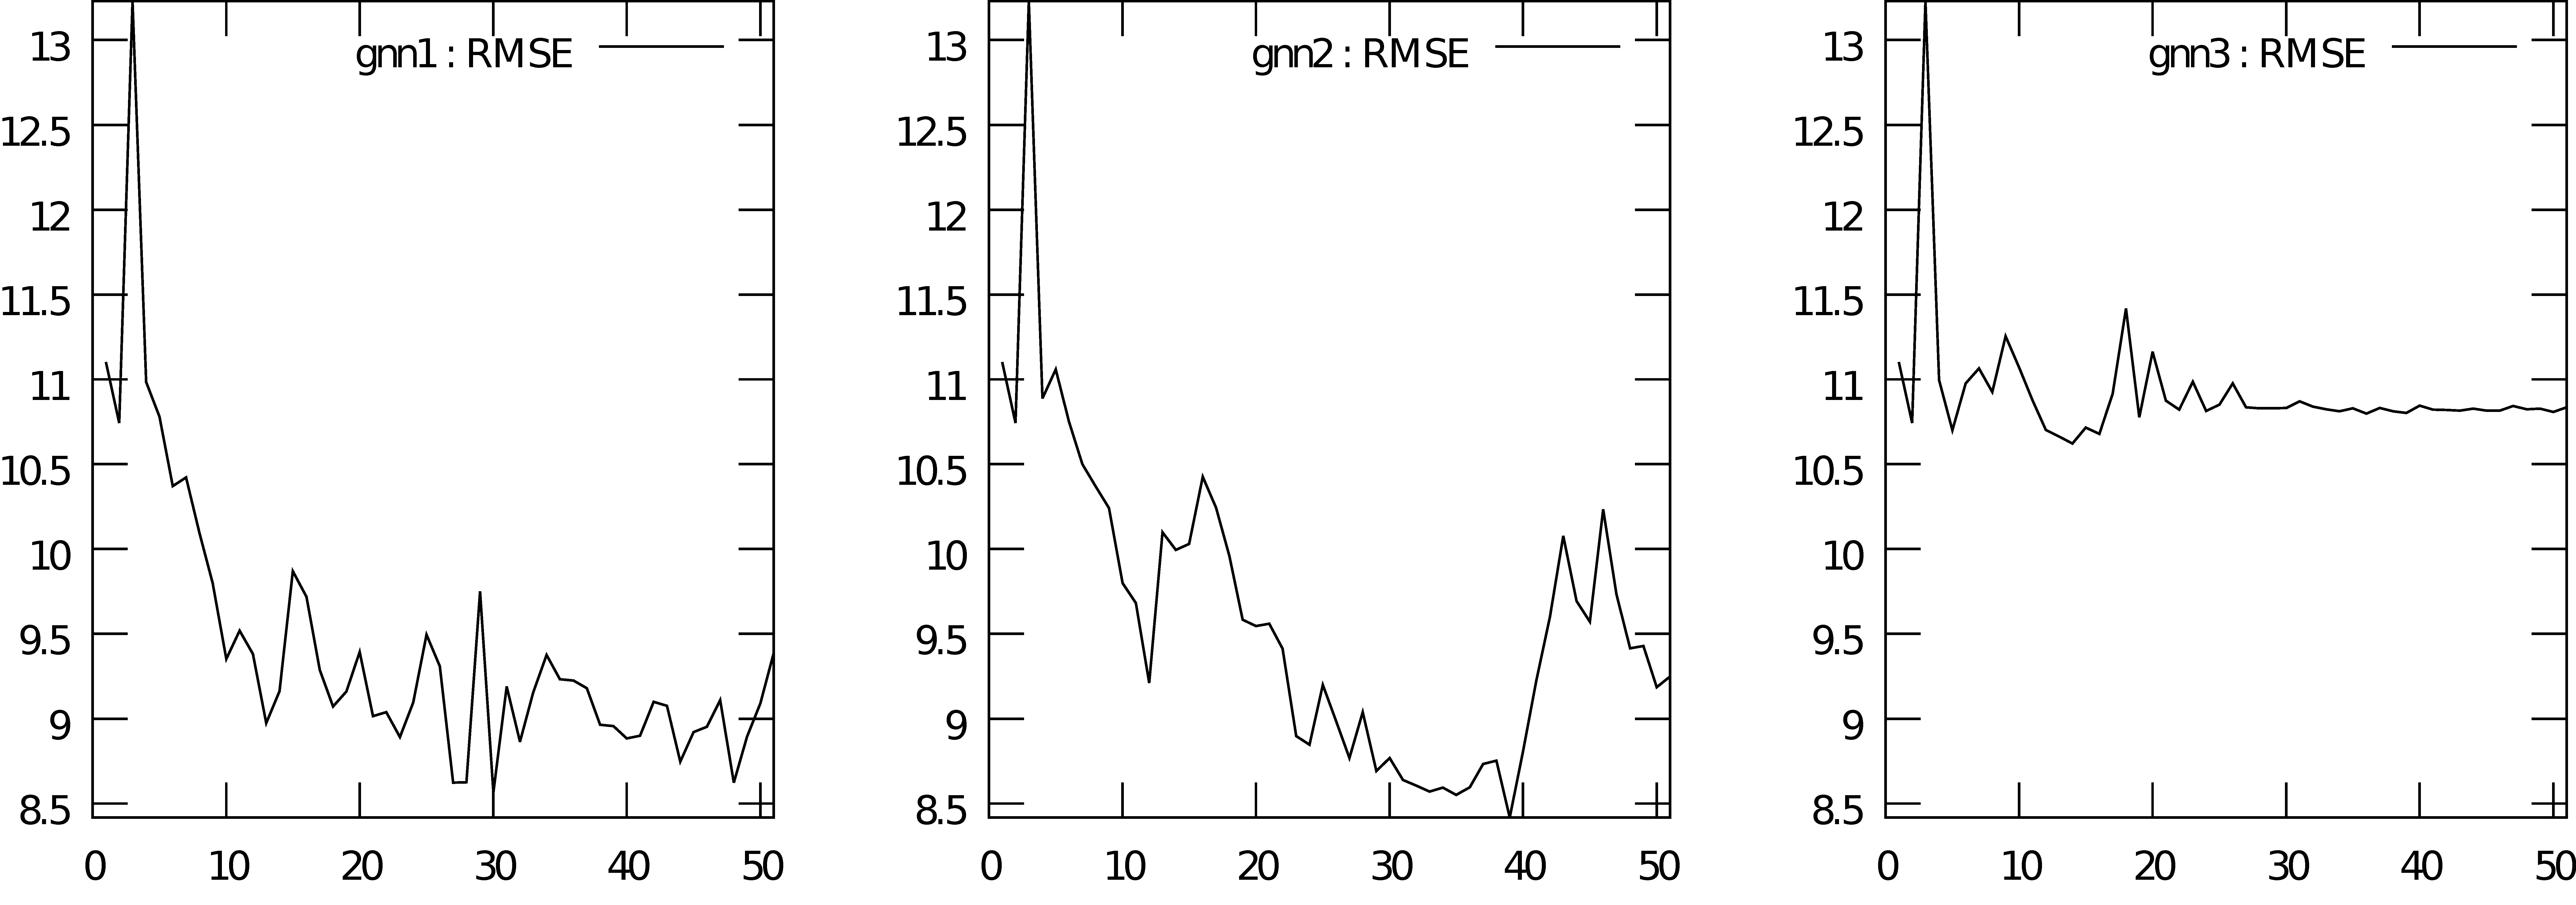
\includegraphics[scale=0.07]{img/rmse1_clipped}
	\caption{GNN performance with $\mu \in [1.2, 0.9, 0.6]$}
	\label{fig:rmse}
\end{center}
\end{figure}

\begin{figure}[h!]
\begin{center}
	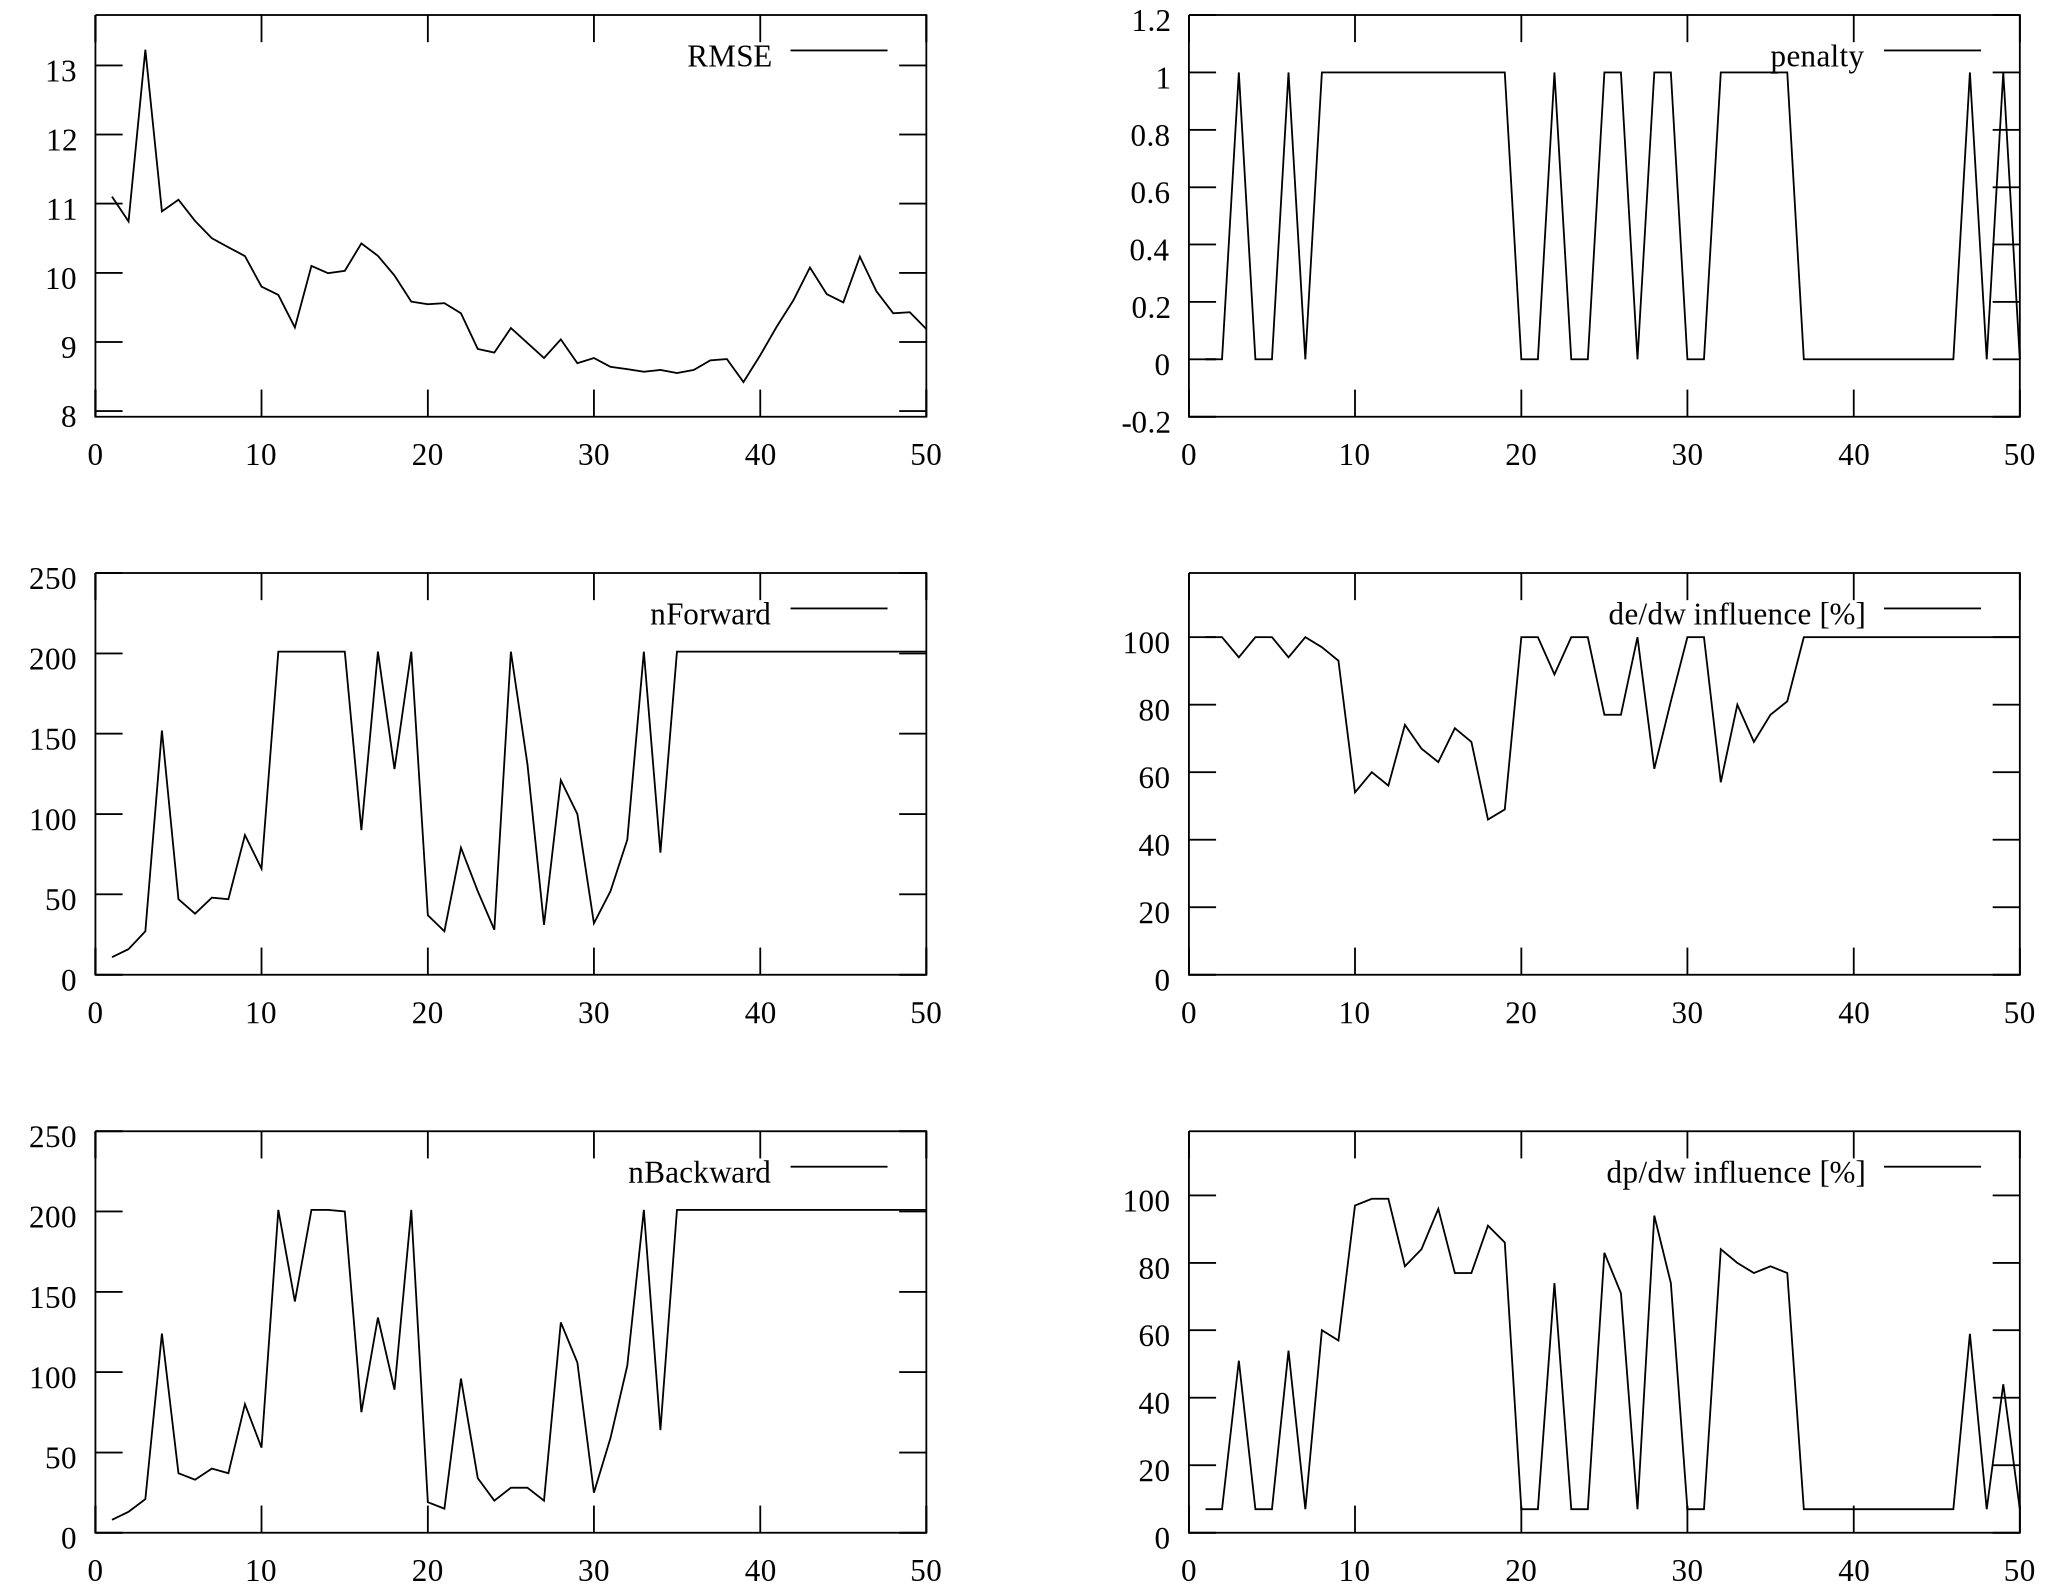
\includegraphics[scale=0.075]{img/gnn1_2}
	\caption{GNN performance with $\mu = 0.9$}
	\label{fig:rmse1}
\end{center}
\end{figure}

\begin{figure}[h!]
\begin{center}
	\includegraphics[scale=0.075]{img/gnn1_3}
	\caption{GNN performance with $\mu = 0.6$}
	\label{fig:rmse3}
\end{center}
\end{figure}

\section{Sample results}
To check if the implemented classifier yields results comparable with these described in the original article~\cite{scarselli2009graph}, another subgraph matching experiment was conducted. Dataset consisted of 100 connected random graphs, each consisting of 14 nodes (node labels in [0..10] edge probability 0.2), the subgraph inserted consisted of 7 nodes. Gaussian noise with zero mean and $0.25$ standard deviation was added to node labels. A 5-fold crossvalidation was performed on the dataset, using a random GNN (five $tanh$ hidden neurons in both computation units, state size 5) with $\mu = 0.9$. For comparison, a 5-fold crossvalidation was performed on the node labels using a feed-forward neural network (inputs, 20 hidden $tanh$ neurons, one output $tanh$ neuron) from the Octave Neural Networks package (10 random FNNs, the one with best crossvalidation results was selected). The results are presented in Table~\ref{tab:crossmean} and Table~\ref{tab:crossstd}. The GNN clearly outperformed the FNN, as it took into account not only node labels, but also graph topology. The obtained results are comparable with the ones from the original article.

\begin{table}[h!]
	\begin{center}
	\begin{tabular}{llll}
	\toprule
	& accuracy & precision & recall \\
	\midrule
	FNN - tr &	75\% &  68\% &  93\% \\
	FNN - tst &	74\% &  68\% &  93\% \\
	GNN - tr &	91\% &  87\% &  97\% \\
	GNN - tst &	91\% &  86\% &  97\% \\
	\bottomrule
	\end{tabular}
	\caption{Mean values on training and test sets}
	\label{tab:crossmean}
	\end{center}
\end{table}

\begin{table}[h!]
	\begin{center}
	\begin{tabular}{llll}
	\toprule
	& accuracy & precision & recall \\
	\midrule
	FNN - tr &	0.68\% &  0.82\% &  1.43\% \\
	FNN - tst &	3.20\% &  2.89\% &  1.85\% \\
	GNN - tr &	1.62\% &  1.71\% &  2.07\% \\
	GNN - tst &	3.06\% &  3.70\% &  1.39\% \\
	\bottomrule
	\end{tabular}
	\caption{Standard deviations on training and test sets}
	\label{tab:crossstd}
	\end{center}
\end{table}

\section{Conclusion}
Implementation of a GNN requires making a couple important decisions which may affect the quality of the classifier results and the computation time. The use of a GNN for a specific dataset may require tuning the GNN parameters, especially the contraction constant $\mu$. Some observations were made concerning the behaviour of a GNN, depending on the value of its parameters:
\begin{itemize}
	\item The best training effect happens when $F_{\bm{w}}$ remains a contraction map
	\item If $F_{\bm{w}}$ definitely ceases to be a contraction map, there are no training effects
	\item Remaining near the contraction state can still yield good results
	\item A fixed maximum number of Forward/Backward steps can still yield good results
	\item Imposing penalty when it isn't necessary should be avoided
	\item Too large penalties (too small $\mu$) should be avoided
	\item The minimum value of $\mu$ should be tuned for the chosen dataset
	\item The minimum value of $\mu$ can be calculated using a subset of data
\end{itemize}

%%%%%%%%%%%%%%%%%%%%%%%%%%%%%%%%%%%%%%%%%%%%%%%%%%%%%%%%%%%%%
%%%%% References %%%%%

\bibliography{bib/gnn,bib/fnn}
\bibliographystyle{spiebib}   %>>>> makes bibtex use spiebib.bst

\end{document} 
